\documentclass[12pt,letterpaper, onecolumn]{exam}
\usepackage{amsmath}
\usepackage{amssymb}
\usepackage{sidecap}
\usepackage{tabularx}
\usepackage{csquotes}
\usepackage{makecell}
\usepackage{hyperref}
\hypersetup{
    colorlinks=true,
    linkcolor=blue,
    filecolor=magenta,      
    urlcolor=black,
    pdftitle={Overleaf Example},
    pdfpagemode=FullScreen,
}
%\usepackage[left=0.5cm,right=0.5cm,top=0.5cm,bottom=0.5cm]{geometry}
\usepackage[usestackEOL]{stackengine}
%\setstacktabbedgap{1ex} 
\usepackage{tikz}
\usetikzlibrary{decorations.pathreplacing}
\usetikzlibrary{fadings}
\def\layersep{2.5cm}

\usepackage{enumitem}

%\usepackage[shortlabels]{enumitem}
%\usepackage{enumerate}
\usepackage[lmargin=71pt, tmargin=0.8in]{geometry}  %For centering solution box

% \chead{\hline} % Un-comment to draw line below header
\thispagestyle{empty}   %For removing header/footer from page 1

\usepackage{listings}
\usepackage{xcolor}

\definecolor{codegreen}{rgb}{0,0.6,0}
\definecolor{codegray}{rgb}{0.5,0.5,0.5}
\definecolor{codepurple}{rgb}{0.58,0,0.82}
\definecolor{backcolour}{rgb}{0.95,0.95,0.92}

\lstdefinestyle{mystyle}{
    backgroundcolor=\color{backcolour},   
    commentstyle=\color{codegreen},
    keywordstyle=\color{magenta},
    numberstyle=\tiny\color{codegray},
    stringstyle=\color{codepurple},
    basicstyle=\ttfamily\footnotesize,
    breakatwhitespace=false,         
    breaklines=true,                 
    captionpos=b,                    
    keepspaces=true,                 
    numbers=left,                    
    numbersep=5pt,                  
    showspaces=false,                
    showstringspaces=false,
    showtabs=false,                  
    tabsize=2
}

\lstset{style=mystyle}




\begin{document}



\newtheorem{theorem}{Theorem}[section]
\newtheorem{problem}{Problem}
\newtheorem{proposition}{Proposition}[section]
\newtheorem{lemma}{Lemma}[section]
\newtheorem{corollary}[theorem]{Corollary}
\newtheorem{example}{Example}[section]
\newtheorem{definition}[problem]{Definition}

\newcommand{\BEQA}{\begin{eqnarray}}
\newcommand{\EEQA}{\end{eqnarray}}
\newcommand{\define}{\stackrel{\triangle}{=}}
\bibliographystyle{IEEEtran}
\raggedbottom
\setlength{\parindent}{0pt}
\providecommand{\mbf}{\mathbf}
\providecommand{\norm}[1]{\lVert#1\rVert}
\providecommand{\pr}[1]{\ensuremath{\Pr\left(#1\right)}}
\providecommand{\qfunc}[1]{\ensuremath{Q\left(#1\right)}}
\providecommand{\sbrak}[1]{\ensuremath{{}\left[#1\right]}}
\providecommand{\lsbrak}[1]{\ensuremath{{}\left[#1\right.}}
\providecommand{\rsbrak}[1]{\ensuremath{{}\left.#1\right]}}
\providecommand{\brak}[1]{\ensuremath{\left(#1\right)}}
\providecommand{\lbrak}[1]{\ensuremath{\left(#1\right.}}
\providecommand{\rbrak}[1]{\ensuremath{\left.#1\right)}}
\providecommand{\cbrak}[1]{\ensuremath{\left\{#1\right\}}}
\providecommand{\lcbrak}[1]{\ensuremath{\left\{#1\right.}}
\providecommand{\rcbrak}[1]{\ensuremath{\left.#1\right\}}}
\let\vec\mathbf

\newlist{mydesc}{description}{1} % create a new list called mydesc, of type "description"
\setlist[mydesc]{
  align=left, % use the align-format defined above
  leftmargin=0pt, % indentation for all the lines
  labelindent=1em, % horizontal space before label
  labelsep=0pt
   % horizontal space after label -- set to zero because we add space via "leftwithbar"
}



\begingroup  
    \centering
    
    \LARGE Weekly Report 1-Decision Tree \\[0.5em]
    \large \today\\[0.5em]
    \large Ganji Varshitha\par
    \large AI20BTECH11009\par
\endgroup
\rule{\textwidth}{0.4pt}
\pointsdroppedatright   %Self-explanatory
\printanswers
\newcommand\Solution{
  \textbf{Solution:}\\}
\newcommand{\myvec}[1]{\ensuremath{\begin{bmatrix}#1\end{bmatrix}}}
 %Replace "Ans:" with starting keyword in solution box

\subsection*{Introduction}
It is a supervised classification and regression ml algorithm which is non parametric. It is a hierarchical model and composed of internal decision nodes and terminal nodes.
\subsection*{Algorithm}
The algorithm follows divide and conquer strategy as a test is applied to the input at each node and a branch is selected based on the outcome of the test. Since the rules are in terms of If Else statements it has high interpret-ability.
There are two types of trees :
\begin{itemize}
\item Univariate trees : It uses single input dimension for split and  for numeric attribute it results in binary split where as discrete attribute it results in multi-way split.
\item Multivariate trees: It can use multiple attributes for splitting.
\end{itemize}
Goodness of the split is quantified by impurity measure of the node. If the node is pure, all the instances in that node will belong to the same class.\\
For node m, N$_{m}$ instances reach m, N$^{i}_{m}$ belong to C$_{i}$
\begin{align}
\hat{P}(C_i | \vec{x},m) \equiv p^i_m = {}& \frac{N^i_m}{N_m}
\end{align}
$\therefore$ If the node is pure, $p^i_m $ should be equal to 1 or 0.
Impurity is measured by entropy. Entropy of a node is given by
\begin{align}
I_m ={}& -\sum_{i=1}^K p^i_m \log_2{p^i_m}
\end{align}
where K is number of classes of output.\\
If the node is not pure, we recursively split to decrease the impurity of the node.\\
 N$_{mj}$ of N$_{m}$ take branch j. N$^i_{mj}$ belong to C$_i$
 \begin{align}
 \hat{P}(C_i | \vec{x},m,j) \equiv {}&p^i_{mj} =  \frac{N^i_{mj}}{N_{mj}}\\
 \acute{I_m} = -\sum_{j = 1}^n\frac{N_{mj}}{N_{m}}{}&\sum_{i=1}^K p^i_{mj} \log_2{p^i_{mj}}
 \end{align}
 $\acute{I_m}$ is the expected reduction in impurity after split which is known as \\\textbf{Information Gain}.\\
 $\therefore$ We need to chose attribute which maximises the information gain at each split.\\
Other common measure of impurity is gini index.
\section*{Key points}
\begin{itemize}
\item The algorithm does not work well for linear data but if the relationship between input variable and target is non linear or complex, it will outperform the linear models.
\item The model is highly prone to over-fitting and sensitive to outliers like noisy training instances.
\item It also suffers excessive generalization error.
\end{itemize}
\section*{Unique points}
\begin{itemize}
\item It is a discriminative model.
\item Does not require normalization of inputs
\item \textbf{Learning is greedy!} It splits to get maximum information gain recursively.
\item Training and predicting the data is fast as we only store the parameters of node to split instead of entire training data.
\end{itemize}
\section*{Pruning}
To reduce overfitting, we prune the decision tree.It can be done in 2 ways:
\begin{itemize}
\item Pre-pruning : We declare max depth and stop the node to split and make it a leaf node.
\item Post-pruning: Pruning the sub trees after generating the whole tree. One common way is to prune the lower ends of tree that result in least information gain.
\end{itemize}
\begin{align}
\text{Gini index } = {}& 1-\sum_{j= 1}^c p_j^2
\end{align}
\begin{figure}[!h]
\caption{Algorithm to generate decision tree}
\centering
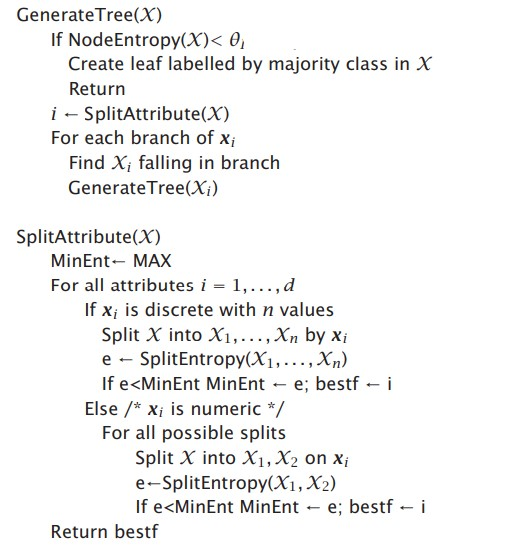
\includegraphics[width = 0.5\textwidth]{../images/tree_gen.jpg}
\end{figure}
\newpage

\subsection*{Questions}

\begin{questions}
\question[] Pick the correct choice.
\begin{choices}
    \choice Pre-pruning is faster, post-pruning is accurate
    \choice Post-pruning is faster, pre-pruning is accurate
  \end{choices} 
  \question[] Information gain \rule{2cm}{0.15mm} at each node.
  \begin{choices}
    \choice Maximised
    \choice Minimised
  \end{choices} 
 \question[]Let $\phi(p_1,p_2)$ be the function measuring impurity of a split. Which of the following is false?
   \begin{choices}
    \choice $\phi(0,1)=\phi(1,0) = 0$
    \choice $\phi(1/2,1/2) \geq \phi(p,1-p)$ , p $\in$ [0,1]
    \choice $\phi(p,1-p)$  is decreasing in p on [0,1/2]
    \choice $\phi(p,1-p)$  is decreasing in p on [1/2,1]
  \end{choices} 
  \question[] Do we require normalization of features while training the model?\\
  \begin{oneparchoices}
    \choice Yes
    \choice No
  \end{oneparchoices}
  \question[] If the measure of impurity is gini index,the feature with \rule{2cm}{0.15mm} gini index is selected.\\
  \begin{oneparchoices}
    \choice Highest
    \choice Least
  \end{oneparchoices}
  
\end{questions}







\end{document}